\subsection{Prime-Time Ratio} \label{subsec:primetime}

ISPs design networks to handle peak demand, which is usually observed
during prime-time hours, when subscribers heavily consume real-time
entertainment traffic, such as video.  The FCC defines prime-time as the
local time from 7:00--11:00 p.m.~\cite{fcc2014measuring-broadband}. To
measure the concentration of network usage during prime-time, we use
Sandvine's definition of the \emph{prime-time ratio}: the ratio of the
average (hourly) traffic demand during prime-time hours to the average
demand in non-prime-time hours~\cite{sandvine20141h, sandvine20142h}.
We measured the prime-time ratio of the subscribers in the control and
treatment groups considering each contiguous four-hour period in each
day. Our experiment shows that, in fact, the evening hours with the
largest prime-time ratio are 8:00~p.m.--12:00~a.m., so we use this time
interval for our definition of prime time.

%\begin{figure}[t]
%\begin{minipage}{1\linewidth}
%\centering
%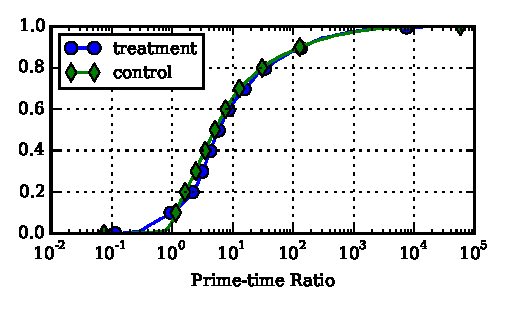
\includegraphics[width=1\linewidth]{figures/prime-time-ratio-per-device-cdf-MEAN.pdf}
%\caption{Prime-Time Ratio\label{fig:cdf-prime-time-ratio}}
%\end{minipage}
%\end{figure}

%\begin{subfigure}[]{.32\linewidth}
%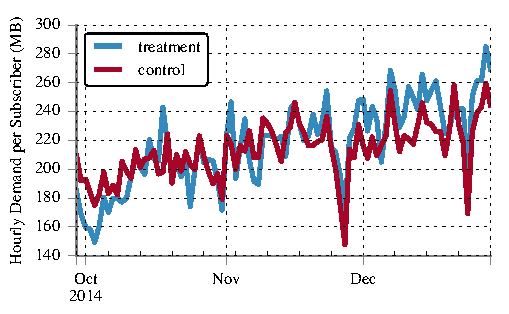
\includegraphics[width=1\linewidth]{figures/primetime_usage_per_day_per_subs.pdf}
%\caption{\label{fig:pt}}
%\end{subfigure}

%\begin{subfigure}[b]{.32\linewidth}
%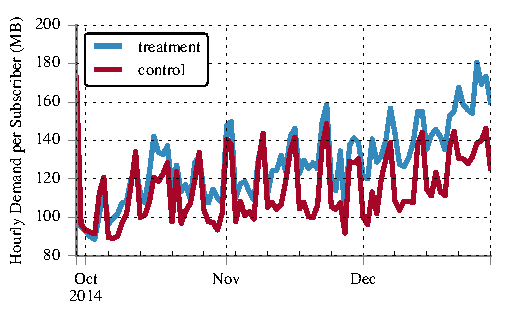
\includegraphics[width=1\linewidth]{figures/nonprimetime_usage_per_day_per_subs.pdf}
%\caption{\label{fig:non-pt}}
%\end{subfigure}

\begin{table}[t]
\centering
\begin{tabular}{cc|c|c|c|}
\cline{3-5}
                                               &           & \begin{tabular}[c]{@{}c@{}}Hourly traffic\\ in PT\end{tabular} & \begin{tabular}[c]{@{}c@{}}Hourly traffic\\ in Non-PT\end{tabular} & \begin{tabular}[c]{@{}c@{}}Prime-time\\ Ratio\end{tabular} \\ \hline
\multicolumn{1}{|c|}{\multirow{2}{*}{Weekday}} & treatment & 233.12                                                         & 124.18                                                             & 1.88                                                       \\
\multicolumn{1}{|c|}{}                         & control   & 225.40                                                         & 104.30                                                             & 2.16                                                       \\ \hline
\multicolumn{1}{|c|}{\multirow{2}{*}{Weekend}} & treatment & 246.93                                                         & 143.08                                                             & 1.73                                                       \\
\multicolumn{1}{|c|}{}                         & control   & 238.15                                                         & 133.16                                                             & 1.79                                                       \\ \hline
\end{tabular}
\caption{\green{Hourly traffic demand during (and outside) prime-time
    hours per subscriber, in MB. Prime-time traffic demand is defined as
    the average traffic demand during a prime-time
    hour.}\label{tab:prime-time-demand}} 
\end{table}

Table~\ref{tab:data-stats} shows that the average hourly prime-time downstream traffic per
1,000 subscribers is
209.5 GB for the treatment group, compared to 205.1 GB for the control
group, \green{ which is about a 2\% difference.} 
In contrast, during an average hour
{\em outside} of prime time, the traffic per 1,000 subscribers is 122.3
GB for the treatment group, compared to
108.5 GB for the control group, amounting to \green{about a 12\% difference.} The
more significant difference in demand during hours outside of the
daily prime-time is also apparent from the weekly usage patterns in
Figure~\ref{fig:traffic-demand-timeseries}. 

% \sgfoot{ \textbf{Interesting
%     reviewer comment we can add here}: Throughout the paper, I was
%   wondering the extent to which congestion was affecting the results.
%   It's well-known that Comcast and other ISPs over-subscribe their
%   network, relying on statistical multiplexing.  Thus, during peak
%   hours, it may be the case that both control, and treatment groups are
%   receiving the same level of service.  In this case, the results the
%   low level of increase during prime time (2\%) relative to the higher
%   level of increase outside of prime time (12\%) might be explained.  I
%   don't know if the authors can tell the extent to which congestion is a
%   factor given the data, would be in would be an interesting discussion
%   nevertheless.} 


We also calculated the prime-time ratio per day over weekends and
weekdays, as shown in Table \ref{tab:prime-time-demand}.  On weekends,
the prime-time ratios for the treatment and control groups are 1.73 and
1.79 respectively. On the weekdays, the prime-time ratio for the control
group is 2.16 compared to 1.88 for the treatment group. 
In terms of absolute demand, the prime-time demand
on weekdays in the treatment group is within 4\%
of that in the control group. In contrast, the demand in
{\em non-prime-time hours} is 19\% higher for the treatment group on weekdays,
and only 7.5\% higher on weekends. \red{The large difference in non-prime-time
demand between the control and treatment groups on weekdays suggests
that many of the users in the treatment group may in fact be subscribers
who work from home may adjust their behavior during non-prime-time hours
and weekdays in response to a higher service tier.}

Although 6\% of the subscribers in both groups had a prime-time ratio over
100, we also observed that 9\% of the control group and 14\% of the
treatment group had prime-time ratios {\em less than one}, indicating that
these users actually had higher demand during the day than they did
during prime time. Similarly, these users may be small home
businesses or subscribers who work at home.


%\if 0
%For our dataset, the prime-time ratio for the treatment and control groups
%were 1.70 and 1.93 respectively. By definition, the prime-time ratio is measured using
%total traffic volume in a day. However, not all subscribers contribute equally
%to the traffic volume. We observed that the median \emph{prime-time ratio per subscriber}
%is 3.39 for the \treatment{} group and 2.91 for the \control{} group. 
%The prime time ratio of the higher tier is more than the lower tier when calculated per
%subscriber, but by volume it is the inverse.
%The overall demand of subscribers in \treatment{} has increased substantially
%on a per-subscriber basis, although the total volume does not show the same increase.
%This result indicates that individual subscribers that do not contribute substantially
%to the traffic volume are the ones who have higher usage in prime-time as compared to their
%lower tier counterparts.
%\fi

